\documentclass[AutoFakeBold]{LZUThesis}

\begin{document}
\title{{建党100周年以来河南红色基因传承弘扬状况调研}}
\author{李文涛}
\major{电子信息基地班}
\kahao{320200928101}
\advisor{赵发琪}
\college{信息科学与工程学院}
\grade{2020}



\maketitle
\frontmatter

%中文摘要
\ZhAbstract{
    2021年,是我们中国人民共产党成立的100周年,在我们党的领导下,全国人民在发展之路上筚路蓝缕,交出了傲人的中国答卷。在脱贫攻坚、改革开放、生态文明建设等方面取得了伟大胜利。在发展的过程中,无数优秀红色精神不断涌现,红色基因就是中国共产党人和中国人民在长期奋斗中形成的伟大精神,习总书记曾讲,“红色江山来之不易,守好江山责任重大。要讲好党的故事、革命的故事、英雄的故事,把红色基因传承下去,确保红色江山后继有人、代代相传” \cite{xjp}。在新时代中国的发展过程中,红色基因的传承和发扬是我们保持文化自信,坚定走中国特色社会主义道路的定心针,定能够成为中国特色社会主义道路建设的一大助力。
        
    
    
    我们党中央高度重视红色基因的传承和发扬,时刻提醒我们不忘前辈们给我们留下的宝贵经验,积极开展红色基因宣传。在我们身边就有许多红色精神的文化载体,但随着社会的发展,不乏不和谐的出现数典忘祖的声音。
    作为新时代的大学生,不仅要做到自我能力技术过硬,还要加强自我精神文化的建设。为了能够更好地加深自己对在思想政治课中学习到的理论的理解,并提高自己的社会实践能力,我组织同学组成“红色中原行”实践调研队回到了家乡河南进行了实地调研,了解在该地区的红色基因的传承和发扬情况,为家乡的红色文化传承贡献一份自己的力量。}
{红色文化、传承、发扬、河南、调研}

%英文摘要
\EnAbstract{The year 2021 marks the 100th anniversary of the founding of the People's Communist Party of China (CPC). Under the leadership of the CPC, the Chinese people have made proud achievements in trailblazing development. Great victories have been achieved in poverty alleviation, reform and opening up, and ecological progress.  We must tell the story of the Party, the story of the revolution and the story of the hero, pass on the red gene, and ensure that the red country will be passed on from generation to generation." In the process of China's development in the new era, the inheritance and development of the red gene is a decisive pin for us to maintain cultural confidence and firmly follow the road of socialism with Chinese characteristics, and will certainly become a major boost for the construction of the road of socialism with Chinese characteristics.

Our Party Central Committee attaches great importance to the inheritance and development of the red gene, always reminds us not to forget the valuable experience left to us by our predecessors, and actively carries out the publicity of the red gene. There are many cultural carriers of the red spirit around us, but with the development of society, there is no lack of inharmonious emergence of the voice of the number classic and forget the ancestor.
    \fontspec{Times New Roman}}
{Red culture, inheritance, development, Henan, research}

%生成目录
\tableofcontents
\thispagestyle{empty}


%文章主体
\mainmatter
\chapter{社会实践情况简述}

\section{积极了解红色文化}
虽然线下进行实地调研收到了阻碍,但我们积极寻找一切其他手段进行红色精神的学习,在原计划中,我们会重点在河南省红旗渠纪念馆及周边,焦裕禄纪念馆及兰考县部分村落,鹤壁市山城区石林会议旧址开展调研,均为河南地区比较著名的红色景点,同时三个地点分布均匀,方便团队成员了解到河南不同地区的红色文化以及当地的社会风貌。在疫情的影响下,我们不能够进行实地调研,但是在我们的努力下,我们和博物馆人员达成联系,在线上进行了相关红色文化的学习。提高大学生个人对我国革命及发展的了解,培养爱国精神,了解我国部分地区在共产党的带领下是如何进行筚路蓝缕的发展,学习他们百折不挠,敢于开创的精神。
\section{调研文化宣传程度}
为了对症下药调查并处理红色文化的宣传情况,我们暑期实践队通过朋友圈、QQ空间等互联网媒介发放红色知识的调查问卷以了解当地居民对红色文化的了解程度。我们的调查问卷共计20道题,涉及有关红色精神的宣传内容、宣传效果、宣传方式等方面,全面地调查目标人群地红色文化宣传情况。

在进行问卷调查过程中,我们总结出但不限于以下几点的调查反馈:大家多红色精神的理解不够全面,对于红色革命精神,大部分人都知道井冈山精神、长征精神、延安精神,而知道大庆精神的人则相对较少。其次,我们需要更多的学习红色精神的渠道,绝大多数人认为以网络短视频、定期组织文化宣讲、影视歌曲广播的方式更利于宣传红色文化,宣扬红色精神。在大家的反馈中,大家对红色精神的认同程度很高,认为革命精神和红色文化在当代依旧有重要的意义,需要发扬好、传承好。同时现在的红色知识普及缺乏趣味性,应设计创新宣传方式,加大宣传力度,从小抓起,让青少年重视这方面的学习。
\section{进行红色文化践行和宣传}
我们召开了以“探访红色景点,发扬红色精神”为主题的线上宣讲活动,制作了关于红色精神的网站,用行动传达红色精神,积极参与到抗洪救灾、抗击疫情的队伍中去。在志愿者行动中,我又一次深深感受到了中华民族骨子里的韧性、越挫越勇,“越是困难重重,越是要迎难而上”。红色精神并不是空有说辞,而是真真正正在当下的疫情大环境下能够作为人们的精神灯塔,指引人们前行的极具实际意义的思想食粮。

在此之后,团队与八月中旬面向当地一所中学学生就中原红色文化进行线上宣讲,积极传播相关红色文化知识,选择思想价值观念尚未成熟的中学生,能够对他们的人生起到正确的引导作用。同时我们积极搭建主题网站,记录团队活动以及进行状况,制作红色宣传影片,在这个信息高度发达的时代用更有效的方式让更多的人认识到红色精神的重要性。
\begin{figure}[htbp]
    \centering
    
\includegraphics[width=300pt]{yanjiang.jpg}
    \caption{宣讲PPT}
\end{figure}
\begin{figure}[htbp]
    \centering
    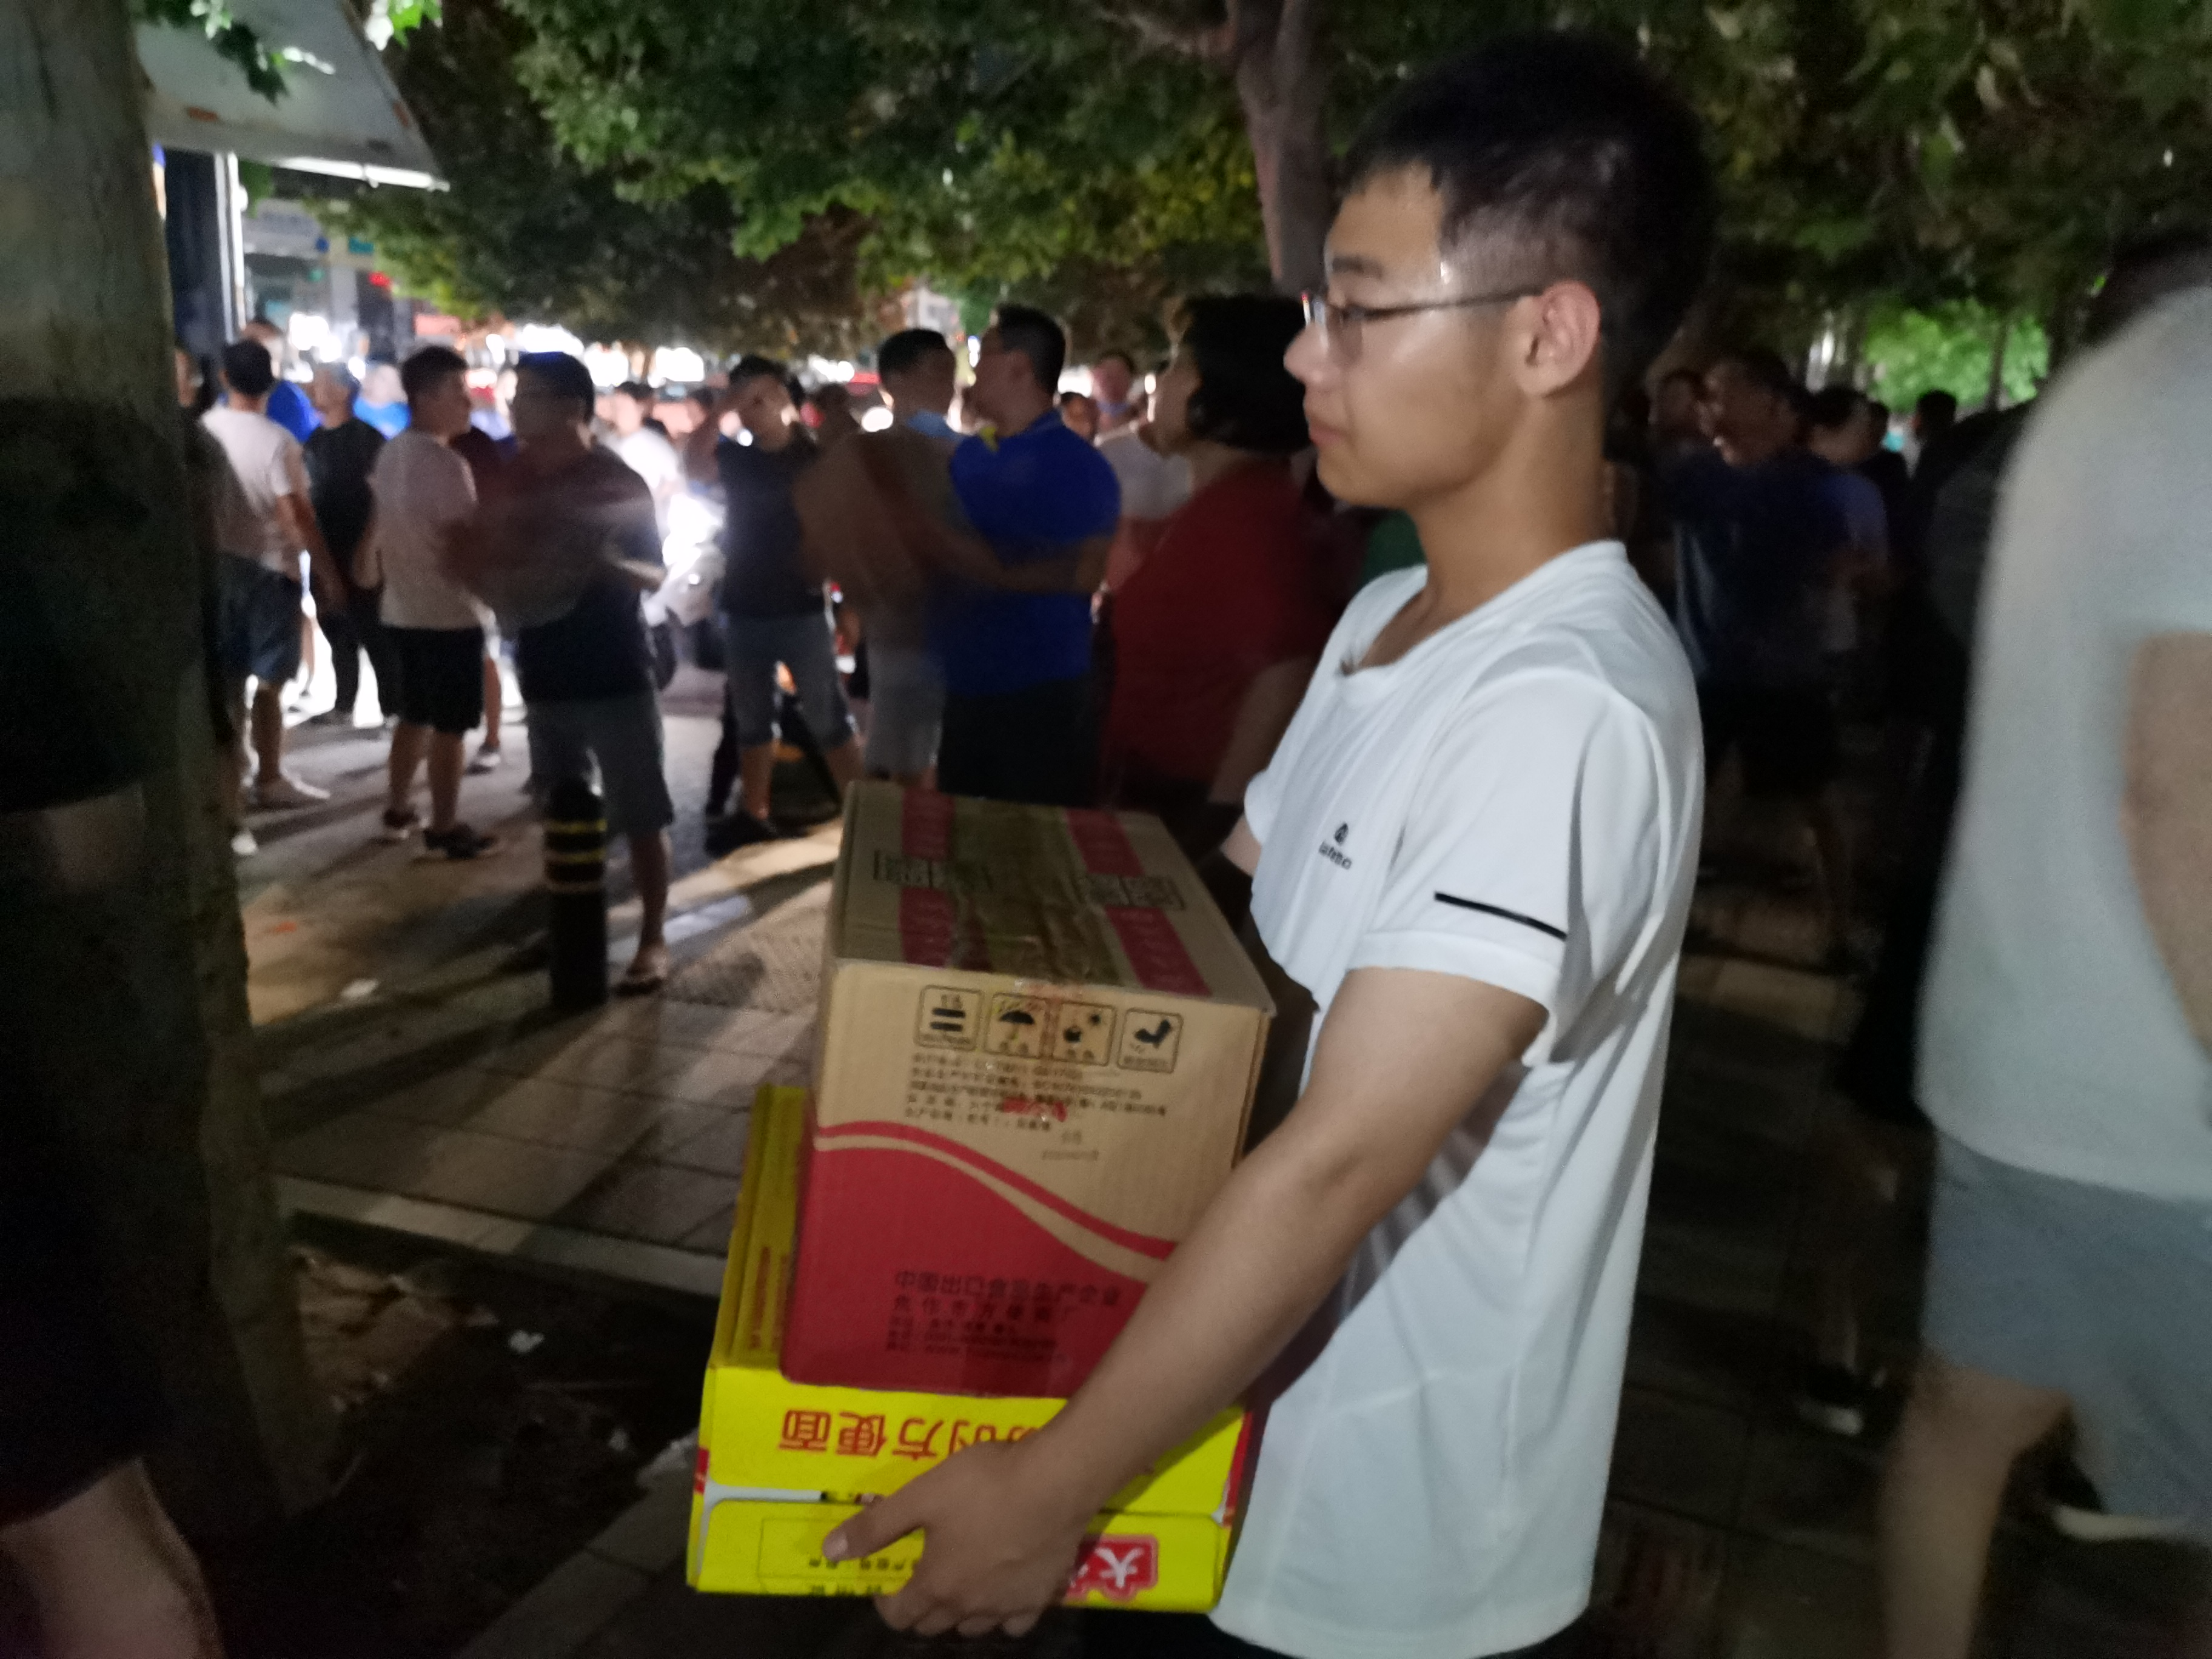
\includegraphics[width=300pt]{kanghong.jpg}
    \caption{我在郑州参与搬运物资时的照片}
\end{figure}
\chapter{调查结果分析}
2021年8月13-17日之间,我们发布问卷并进行收集结果,经过筛选清洗,最后收集了一百余条有效数据,并通过问卷星平台对数据进行了可视化处理,以下基于这些数据分析当地的红色文化宣传和传承情况,并以此做出规划和建议。
\section{受访人群概况}
经年龄分布的饼图(图2.1)可知,受试者中20岁以下的青少年占70\%,符合我们的调查目的,整体倾向于对青少年的红色文化调查和宣传,于此同时年龄分布(图2.2)占第二位的是21-30岁,我们在发布时选取的采样地区在学校附近,涉及人群为学生和教师以及和学校相关的社会人士。调查群体的男女比例为58.18\%:41.82\%,大致上满足男女平衡,样本分布合理,可信度高。


\begin{figure}[htbp]
    \centering
    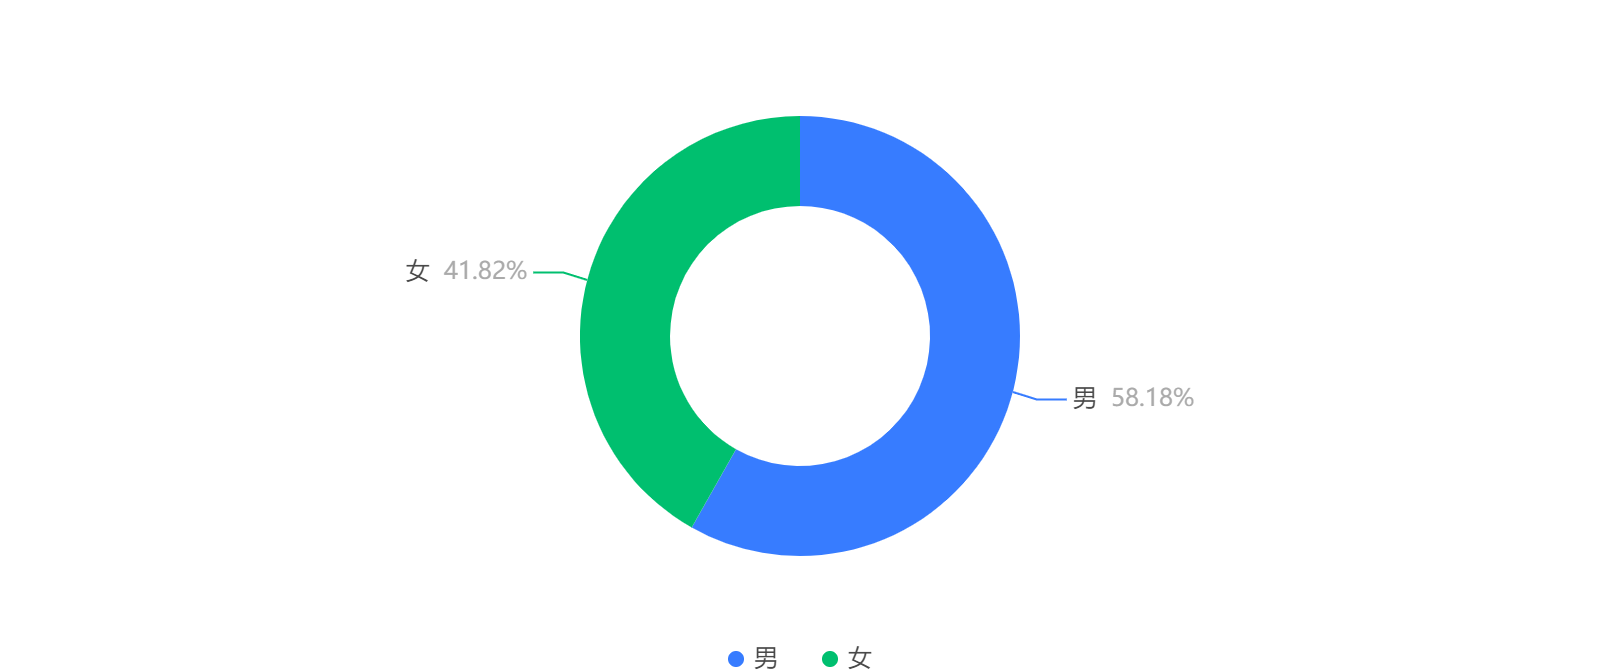
\includegraphics[width=500pt]{sex.png}
    \caption{调查人群年龄分布}
\end{figure}

\begin{figure}[htbp]
    \centering
    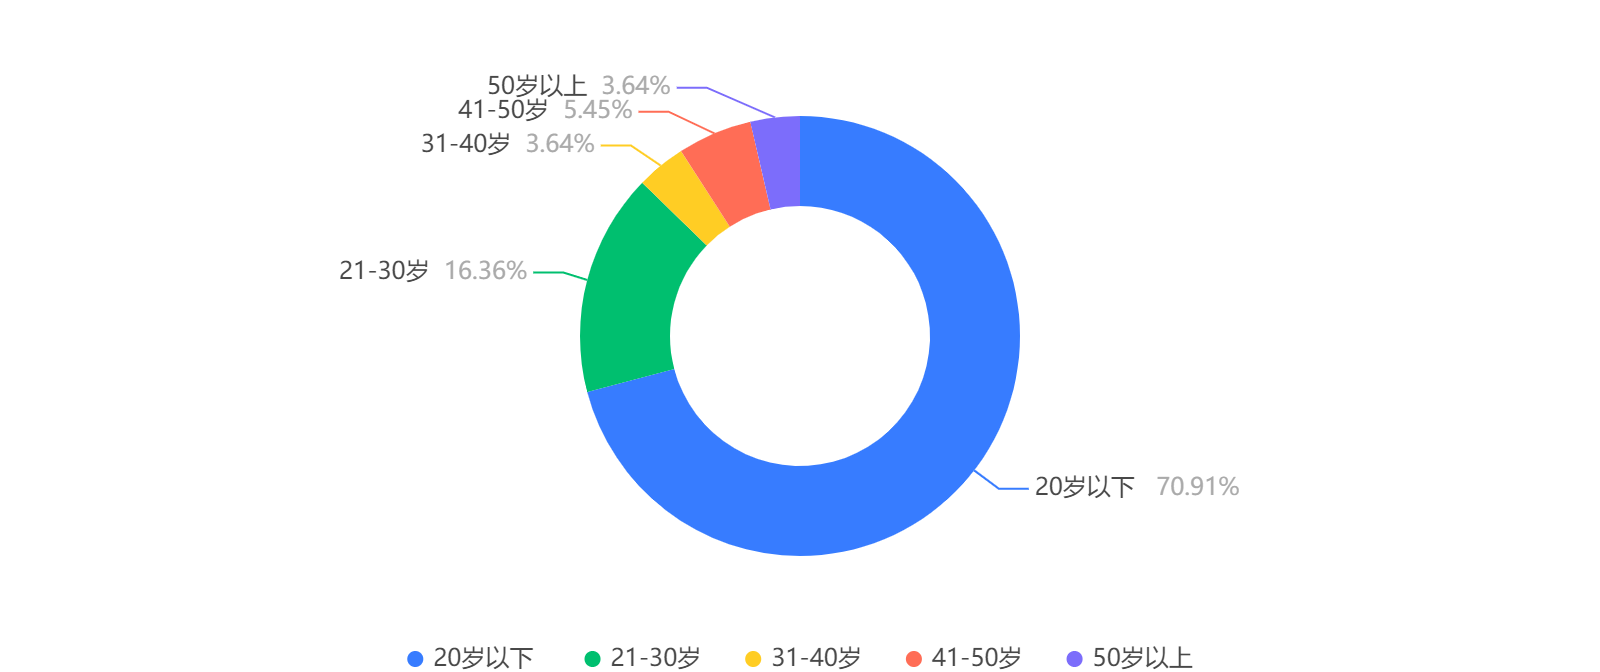
\includegraphics[width=500pt]{age.png}
    \caption{调查人群性别分布}
\end{figure}

\section{受测人群对红色文化的了解程度}

基于目标受访群体,我们设置了具有针对性的问题,进一步分析目标群体对红色文化的了解程度,总结地区的红色基因传承和红色文化宣传的落实情况,为接下来的红色文化宣传规划及方向打好实际情况支持。

\begin{figure}[htbp]
    \centering
    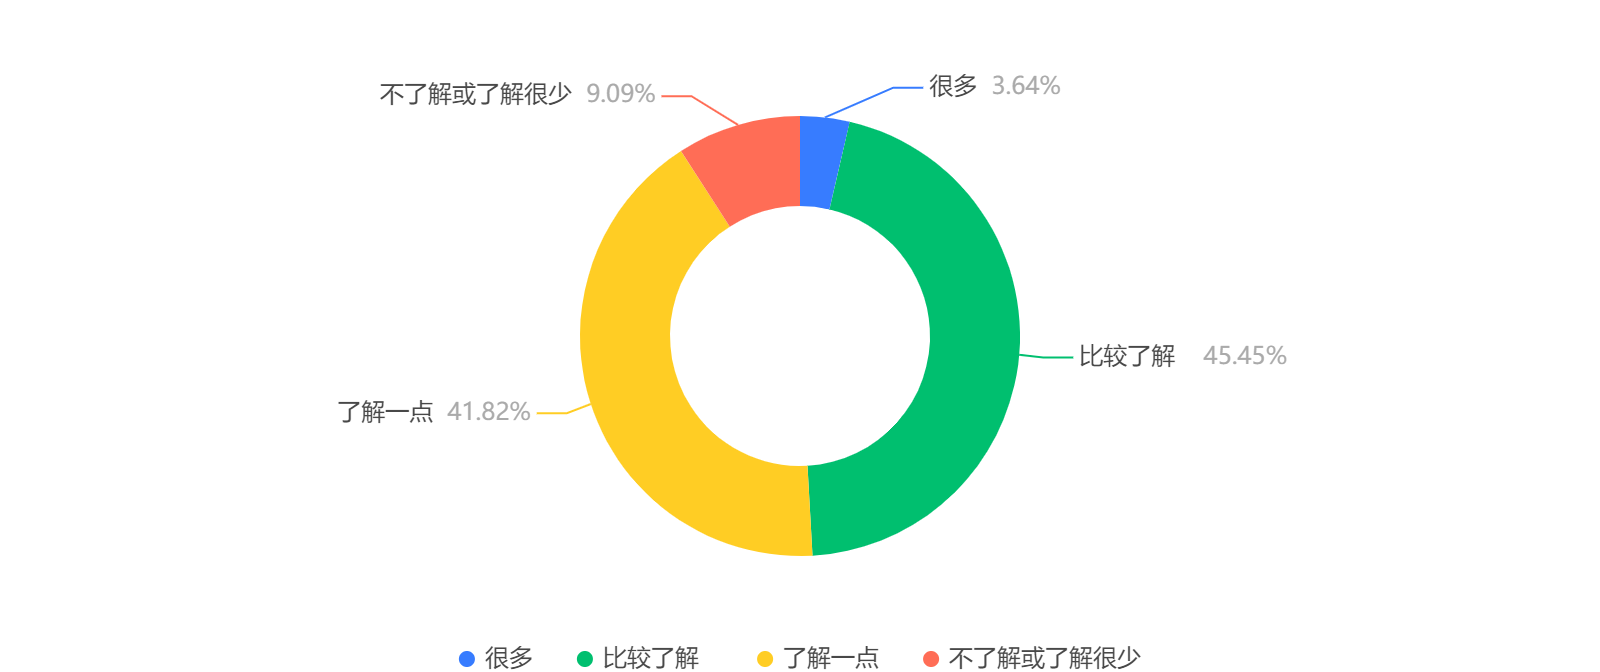
\includegraphics[width=500pt]{shiji.png}
    \caption{受测人群对红色文化的了解程度}
\end{figure}

我们在问卷里设计了几个具有代表性的河南红色精神,内容包括焦裕禄精神、红旗渠精神,同时也涉及几个有广为人知的红色精神,例如井冈山精神、长征精神、延安精神。对于本地的红色文化、革命事迹,其中对这些红色文化十分了解的人占3.64\%,不了解或了解很少的占9.09\%,了比较了解的个体占45.45\%,了解一点的个体占41.82\%。如果大致上以比较了解与了解一点作为第二次分类的分界,人群中具备基本的红色文化知识的只占一半,以此可以大致反映出当地的红色文化宣传工作成效不够明显。

\begin{figure}[htbp]
    \centering
    \subfloat[受测人群对红旗渠精神内涵的认识]{
    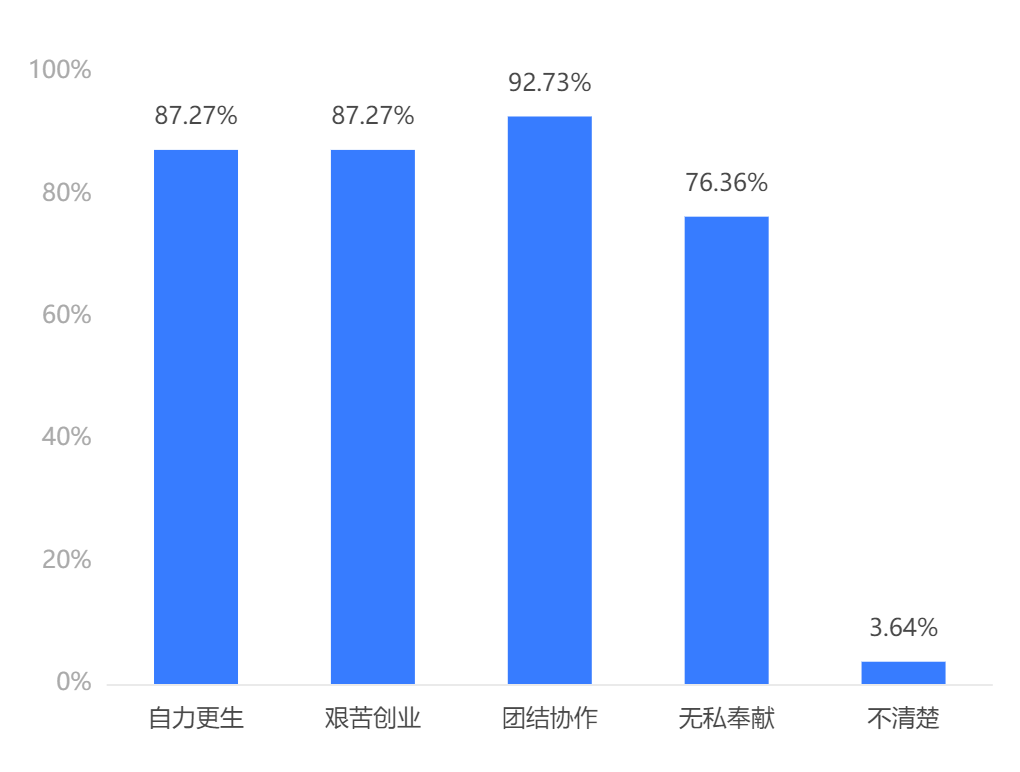
\includegraphics[width=5.5cm]{hongqiqvjs.png}
    \label{(a)}
    }
    \quad
    \subfloat[受测人群对焦裕禄精神内涵的认识]{
    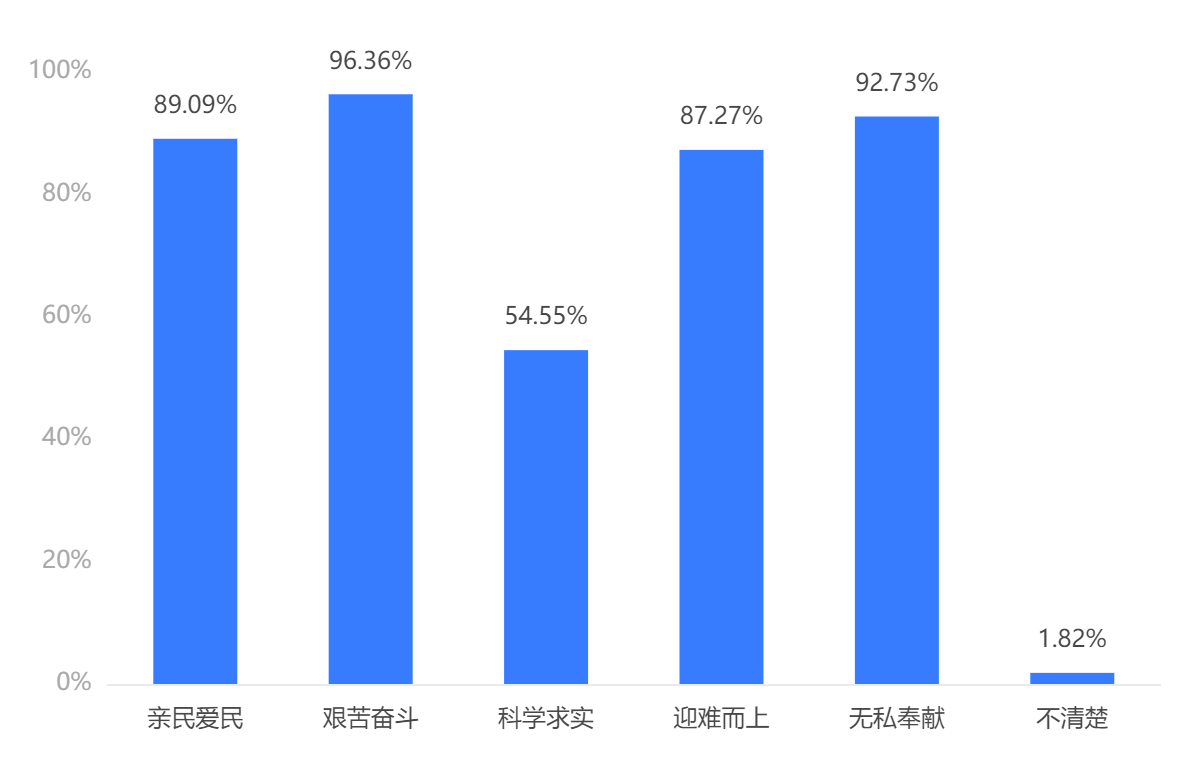
\includegraphics[width=5.5cm]{jiaoyulujs.png}
    \label{(b)}
    }
    \caption{受测人群对红色文化内涵的认识}
\end{figure}

针对河南红色文化中具有代表性的红旗渠精神和焦裕禄精神,我们设置了选择题来调查受测人群对红色精神的实际了解情况。我们设置选项的依据是总书计对这两种精神的高度概括——“亲民爱民,艰苦奋斗,科学求实,迎难而上,无私奉献”的焦裕禄精神; “自力更生,艰苦创业,团结协作,无私奉献”的红旗渠精神。数据显示,大多数人对这两种精神有一定的理解,只有极少数的受试者选择了“不清楚”。两种精神做横向对比,发现大家对红旗渠精神较为了解,每个概括精神特点的成语都有75\%以上的选择率,而在对焦裕禄精神的理解上,只有54.55\%的受测人群选择了“科学求实”。就总体情况来看,大家对红色文化有一定程度上的理解。

同时对于大众对两种精神理解的横向对比我们猜测与地域有关,在排除“科学求实”这个特例之后,大众理解焦裕禄精神的内涵水平优于红旗渠精神,这也许是因为采样对象所在的长垣市距兰考较近。而我自身也是一个很好的例子,在我的老家河南扶沟坐落着吉鸿昌纪念馆,所以我对这位将军以及他的事迹的了解相对于他人就要更胜一筹。这对于我们进行红色精神宣传有着积极的意义,直接证明了加大宣传力度例如建立纪念馆,让公众在这样的环境下耳濡目染,自然会提高大众对红色文化的理解,也能在平时的一言一行中更好的传承红色精神。

总而言之,受测群体对红色文化的了解程度一般,但大多数人没有对红色精神深入理解,只是听说过相关红色故事,停留在一种浅薄的认识上。如果想让大众真正地了解红色文化的内涵,采取耳濡目染的方法或许是不错的方法。

\section{受访人群对红色文化宣传的感受}
为了针对如何让大众更好地去接受红色精神,理解红色文化内涵,我们设置了一系列对当地红色文化宣传情况的问题,例如,主要包括能否感受到周边的红色文化(图2.5),是否愿意花费时间学习红色文化(图2.6),不关注红色文化的主要原因(图2.7)。前者是考察当地对红色文化的宣传力度,后两个问题可以反应大众对学习红色文化的态度,也可以对症下药,针对大众在面对红色文化时的困扰进行一一解决。

\begin{figure}[htbp]
    \centering
    \subfloat[受测人群对当地红色文化宣传程度的感受]{
    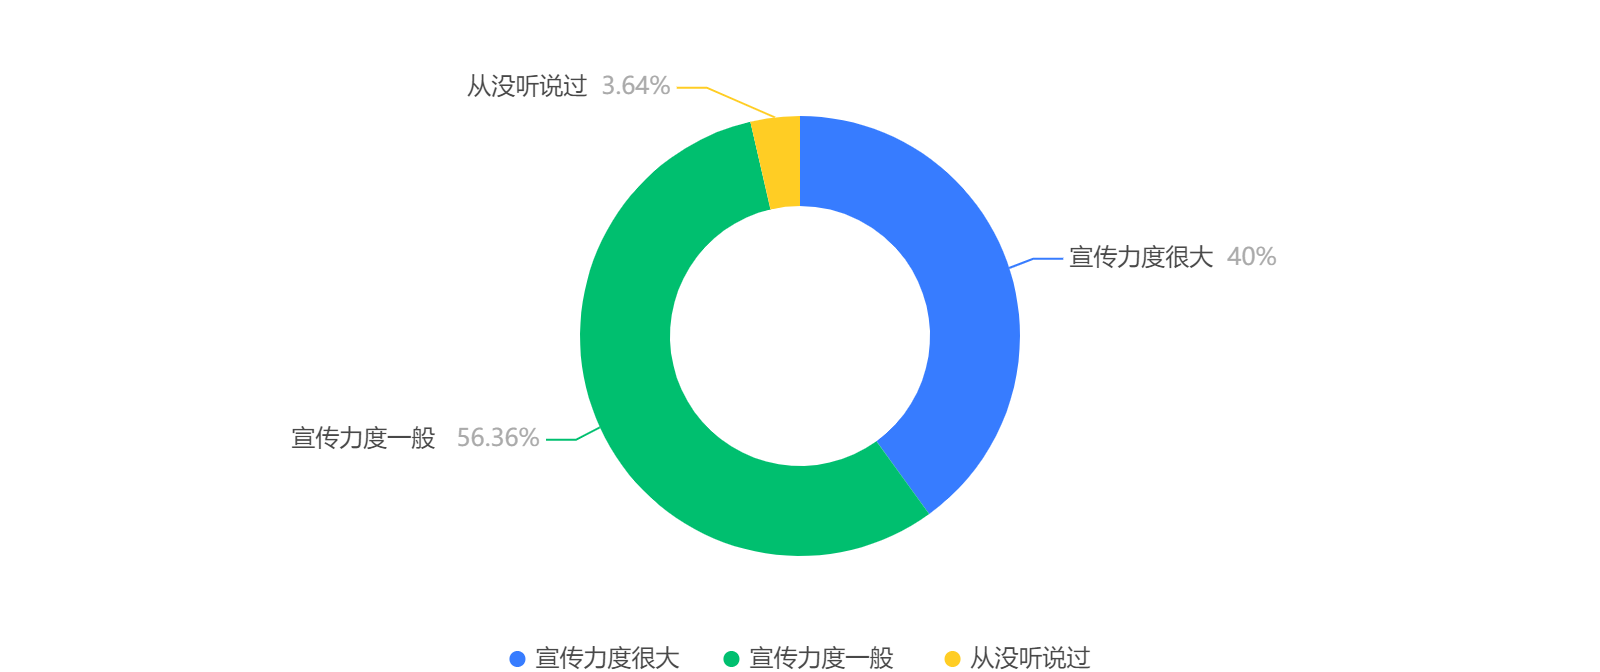
\includegraphics[width=500pt]{xuanchuan.png}
    \label{(a)}
    }
    \quad
    \subfloat[单位或社区举办红色文化宣传活动的频率]{
    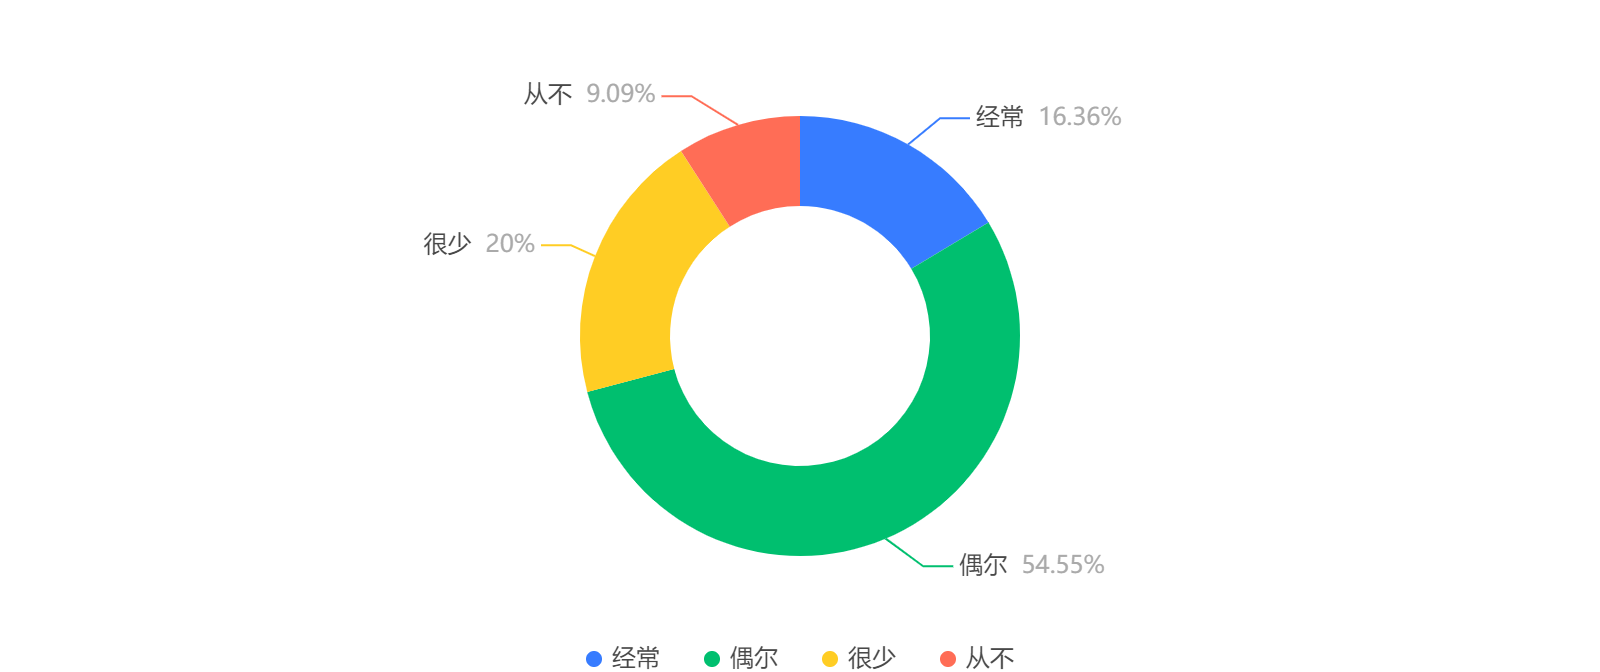
\includegraphics[width=500pt]{juban.png}
    \label{(b)}
    }
    \caption{检测当地红色文化宣传情况}
\end{figure}

由图2.5(a)我们看到只有3.64\%的受测人群选择了“从没听说过”,可以得出当地的红色文化宣传工作的确落实到了,但有56.36\%的受测人群选择了“宣传力度一般”,选择“宣传力度很大”的人数只占40\%,不到总人数的一半,说明落实力度还有所欠缺。
结合图2.5(b)受测人群对单位或社区举办红色文化宣传活动的反馈,选择“从不”的人数占9.09\%,对比图2.5(a)中“从没听说过”的3.64\%,我们猜测大众接受红色文化宣传的来源主要来自单位或社区,反映出当地大型红色文化宣传活动的欠缺。

\begin{figure}[htbp]
    \centering
    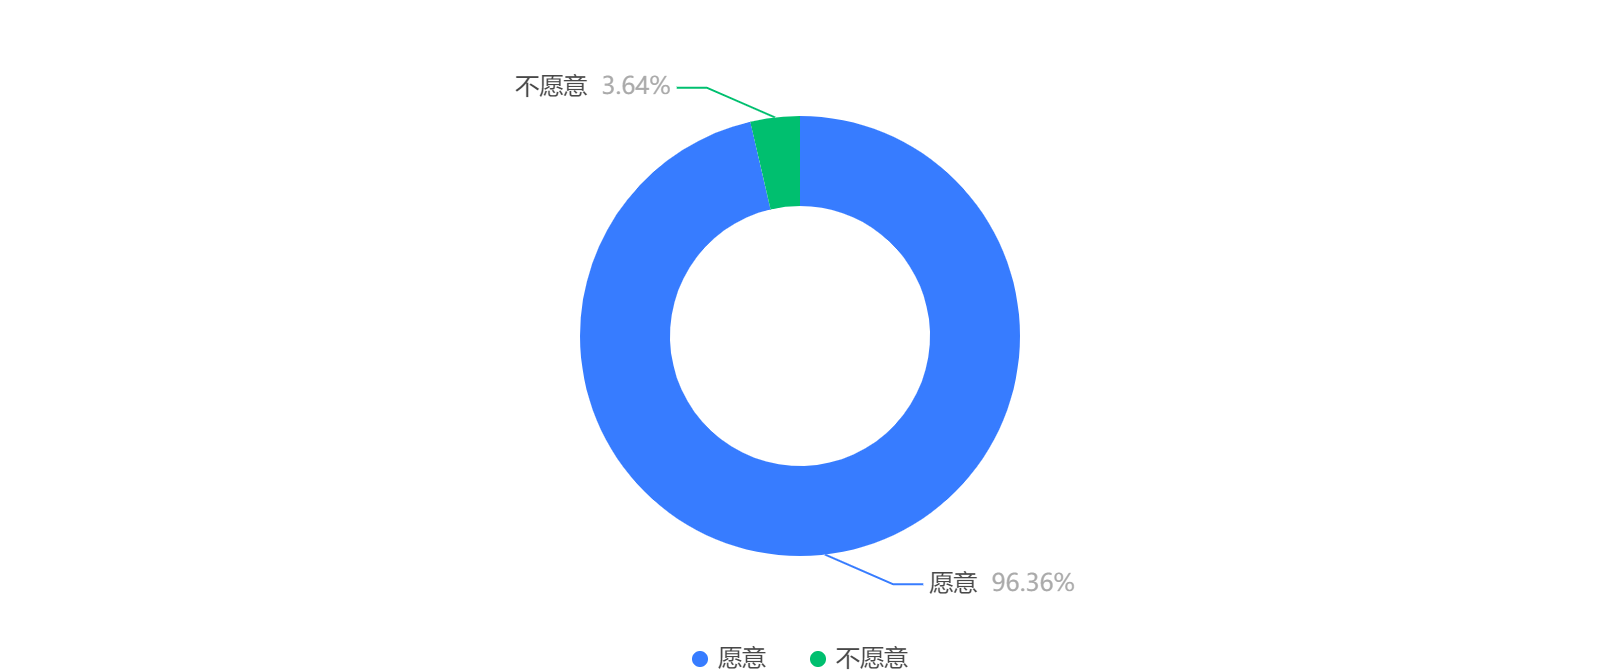
\includegraphics[width=500pt]{zhudong.png}
    \caption{受测人群是否愿意主动学习红色文化}
\end{figure}

接下来我们根据图2.6中的数据可以得到有3.64\%的受测人群选择了不愿意主动学习红色文化、弘扬红色精神,对比图2.5a中的对于红色文化宣传程度的感受情况中有3.64\%选择“从没听说过”,我们猜测对于红色宣传情况的反应一定程度上取决于民众对其的接受度,一些居民如果不愿意去接受红色文化,可能就会出现对红色宣传文化活动的“视而不见”。加上这一因素,我们可以推测当地的红色文化宣传工作落实情况是比较全面到位的。

同时,由图2.6中选择“愿意”的人数占96.36\%也直接说明了当地人民对于红色文化的传承和发扬的态度是十分积极的,大家都乐意去接受并弘扬红色精神,反映了我们党成立100周年以来红色文化宣传的重要性深入人心,民众的民族精神认同感较高。

\begin{figure}[htbp]
    \centering
    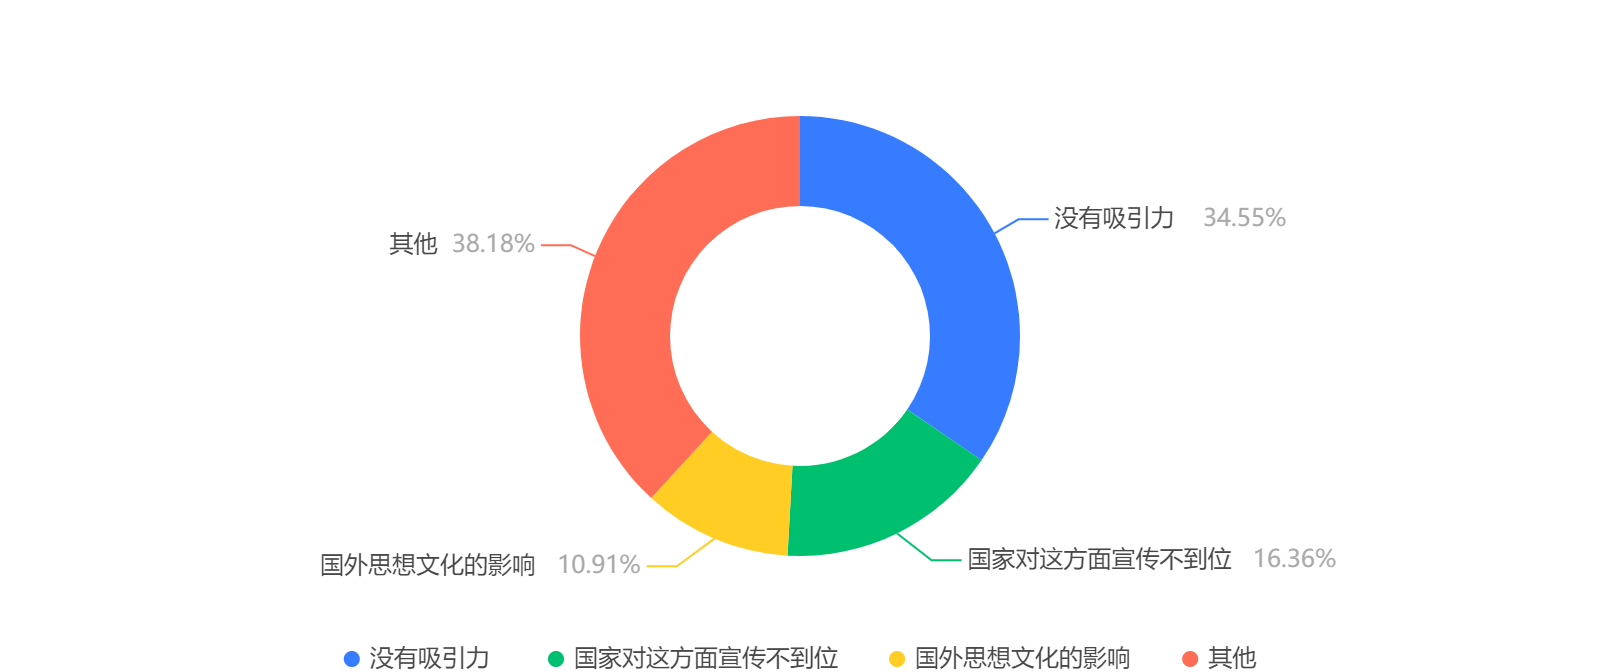
\includegraphics[width=500pt]{buguanzhu.png}
    \caption{受测人群不关注红色文化的主要原因}
\end{figure}

图2.7显示了受测人群对于不关注红色文化的主要原因的反馈,34.55\%的人选择了“没有吸引力”, 16.36\%的人选择了“国家对这方面宣传不到位”,这两点都可以归结于宣传形式或者说是方式不太能够让民众接受,此外还有10.91\%的人选择了“国外思想文化的影响”,这说明崇洋媚外的现象存在一定程度上对红色文化的宣传造成了阻碍。根据这一饼图,我们可以在宣传手段和力度方面做进一步的努力。

\section{受测人群对红色宣传工作的建议}
为了进一步对红色文化宣传工作做出改进,我们向受测人群询问相关情况和意见,比如图2.8(a)调查民众平时是如何了解红色文化的(这里我们以如何学习红旗渠精神为问题对受测人群进行调查),并同时设置填空题向大家征求对于红色文化教育的建议,并根据回答以词云图2.8(b)的形式显示出来。

图2.8数据显示,受众最多的渠道的是“电视报道”,占63.64\%,“听别人介绍”和“网络搜索”受众人数大致相同,均占50.91\%,还有32.73\%的人是由“报纸介绍”来了解红旗渠精神的。而“其他”选项选择占比为0\%,这样我们可以基本推断大众获取红色文化的渠道就限于我们给出的四种方式。同时,“电视报道” 和“听别人介绍”相对于“网络搜索”和“报纸介绍”更倾向一种被动接受红色文化的方法,这部分总占比较大也是一种宣传力度到位的体现。对比“网络搜索”和“报纸介绍”,我们可以知道在信息发达的当下,民众更倾向通过互联网去获取红色文化。

\begin{figure}[htbp]
    \centering
    \subfloat[受测人群了解红旗渠的途径]{
    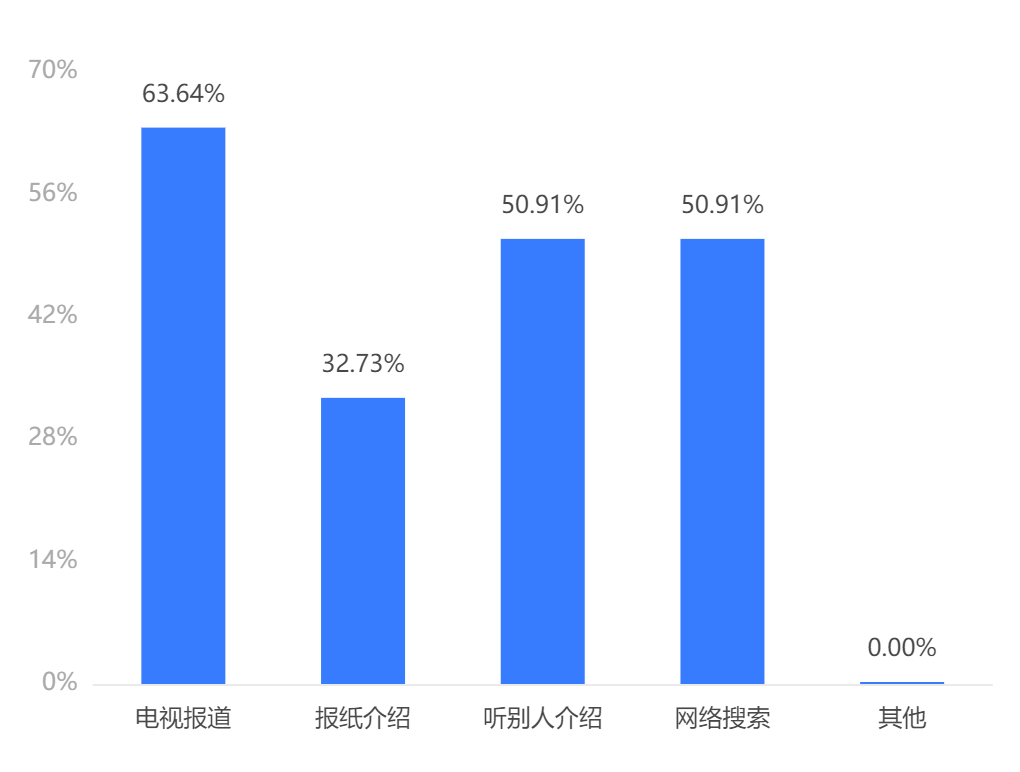
\includegraphics[width=7cm]{tujing.png}
    \label{(a)}
    }
    \quad
    \subfloat[受测人群对进行红色文化教育的建议(词云)]{
    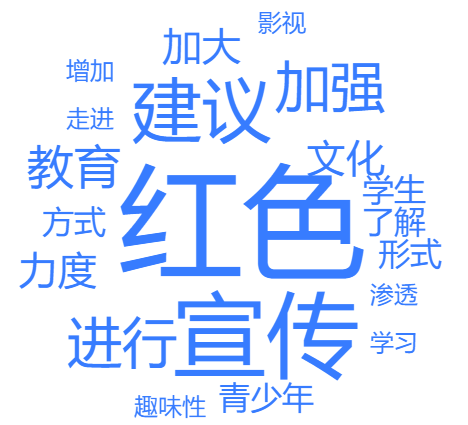
\includegraphics[width=7cm]{ciyun1.png}
    \label{(b)}
    }
    \caption{调查受测人群对红色宣传工作方向的意向}
\end{figure}

词云根据受测者的回答从中选择了出现频率较高的词语,根据频率的不同显示不同的大小。据图2.8(b)显示,“影视、“形式”、“趣味性”这些词反应了大众对于更有趣更多元的红色宣传的接受度更高,希望能够接受到形式更加新颖的红色宣传活动,例如播放红色趣味宣传片,将文字化为视频。政府有关部门应该成立相关融媒体部门制作更多元化的红色文化形式进行宣传。

同时“学生”、“青少年”出现频率较高,表现了大家对红色文化的传承要从小开始的认同较高,这也对我们进行下一步的红色文化宣传工作有了指导性建议,启发了我们以线上会议的方式对学生进行趣味红色文化普及。
\section{调查问卷总结和分析}
根据以上几点对于调查问卷的分析,我们总结了以下几点信息。
\begin{enumerate}
    \item[1.]大家对红色精神的理解不够深入,大多数人只停留在了解相关红色故事的阶段。绝大部分对红色文化的接受意愿高,并对本地的红色文化有一定了解,但只有少部分人了解较深。
    \item[2.]几乎所有人认为有必要在当代传承并主动学习红色革命精神,弘扬红色文化。革命精神和红色文化在当代依旧有重要的意义,需要发扬好、传承好。
    \item[3.]将近一半受测者认为当地红色文化宣传力度一般。政府需要加强大型红色文化宣传活动的组织。
    \item[4.]相对而言,大家还是比较喜欢通过电子媒介的方式获取红色文化。
    \item[5.]从建议来看,现在的红色知识普及缺乏趣味性,应创新宣传方式,加大宣传力度,从小抓起,让青少年重视这方面的学习。
\end{enumerate}
通过调查问卷,我们可以看出我们所调查的地区——长垣市的红色宣传工作比较到位,政府和群众对于红色文化的接受度高,在建党100年以来,红色精神已经扎根于每一个普通民众的心中,大家对于红色文化宣传活动的热情较高,也迫切希望能够看到更有趣的红色宣传活动。
对于以上的分析结果,我建议

\begin{enumerate}
    \item[1.]学校应该多组织同学和老师举办相关了解红色文化的活动。形式上尽可能新颖,能够充分利用互联网环境的优势,例如线上趣味知识问答、组织一起观看红色影片、排演红色小剧场,让红色文化走进校园,让红色精神从小植入每个青年的心中。
    \item[2.]政府应该积极推进红色新媒体的发展,时代在进步,越来越多的人倾向于在网上接受信息,对互联网的信息的接受意愿高。我们改变原有的红色文化宣传方式,宣传当代能够反应红色精神的人和事,制作情景剧、红色元素歌曲等在当下更容易让人接受的宣传媒介,提起民众对红色文化的学习兴趣,让红色文化不再是枯燥的文章,而是在新时代富有活力的精神灯塔。
    \item[3.]鼓励红色景点跟紧新时代,提高自身的影响力,红色景点作为最能集中表现红色文化的地点,应该努力宣传,扩大影响力,利用互联网平台宣传景点的特色,和其他商家联合推出红色周边,让红色文化不再是晦涩的概念,而是能够走进千家万户的元素。
\end{enumerate}

\chapter{红色文化宣传的实践落实}
\section{抗洪与抗疫}
在进行调研时,河南正在遭受疫情和洪灾的考验,作为河南土生土长的一员,我鼓励团队成员积极参与到抗击疫情和洪灾的一线,包括我在内的多名同学都以志愿者的身份参加了不同的抗疫和抗洪的一线,为河南部分地区的灾后重建贡献自己的力量,积极宣传疫情防控相关知识,对社区流动人群进行酒精消毒、体温检测等。

“纸上得来终觉浅,绝知此事要躬行”,我们学习红色精神绝不是空谈,敢于迎难而上、舍己为人才是真正将红色精神内化于心,才能真正地起到传承红色精神的作用。


\section{红色文化宣讲}
为了进一步深入了解红色文化并将其发扬光大。我们与当地中学取得联系并进行协商,于2021年8月15日进行了名为“遍历红色中原,不忘初心使命”的宣讲活动,考虑到我们收集到的红色文化资料,我们选取了“石林会议”,红旗渠精神,焦裕禄精神三个具有典型代表意义的红色文化,分三个部分向同学们普及红色文化知识。

在此次宣讲活动中,我们首先介绍了鹤壁市“石林会议”旧址。每一处遗留下来的红色旧址都在讲述着那段艰苦卓绝、栉风沐雨的岁月。具体向同学们介绍了刘伯承、邓小平等革命先辈挺进大别山的经历。然后是红旗渠的介绍,讲述了林县人民在上世纪60年代不惧困难,迎难而上开辟红旗渠的奋斗史,通过具体事例向同学们介绍红旗渠“自力更生、艰苦创业、团结协作、无私奉献”的精神内涵。接着是兰考县焦裕禄纪念馆,结合焦裕禄的事迹,向同学们介绍了这位人民的好干部在岗位上一心为民、舍己为人的工作态度,深入浅出地分析了焦裕禄精神“亲民爱民、艰苦奋斗、科学求实、迎难而上、无私奉献”的精神内涵。最后联系当下的洪灾和疫情,鼓励大家将红色精神牢记在心,从自己做起,从身边的小事做起,积极投身社会建设,在社会遇到困难时,懂得迎难而上。

\section{多媒体形式宣传}
前文中我不只一次提到了互联网的作用,我们发挥学院特色,将整个调研过程记录在主题网站上供大家浏览,并将线上会议的内容制作成视频投稿在网上供更多的人学习,了解我国红色精神的魅力。

\chapter{收获和感想}
在进行抗洪物资的搬运后,我记录下了当时的感想:

“在参加搬运物资的志愿活动时,大家都热情高涨,没有一个喊累的,'人力传送带'中的人的年龄有小到几岁的,还有上了年纪的老爷爷和老太太,他们寻找着自己能够搬运的东西,做一份自己力所能及的事。我深切感受到河南人民的团结一心和舍己为他的文化精神底蕴,愿受灾地区早日恢复正常,早日完成灾后重建工作。”

通过此次暑期实践学习,我对于红色精神有了更为深刻的理解。在调查当地红色文化宣传地过程中,我深刻感受到了建党100年来我国红色文化的传承,无数的人正以红色精神为导向在新时代的浪潮中披荆斩棘,以全新的故事向我们展示红色精神的生生不息,赋予红色精神新的内涵。民众们都从心底上理解认同红色文化的优越性,积极地参与到红色文化地传承与发扬当中来,这份神奇的默契不禁让我感动,一个民族,无数的人正为了同一个理想,心怀红色精神,在时代的浪潮中交出富有中国特色的答卷,无论什么样的困难都无法将我们打倒,气势汹汹的疫情在我们众志成城的抗疫战线面前也显得苍白无力,这是我们民族自信的体现,是对红色精神的最好诠释。

无论是焦裕禄精神,还是红旗渠精神,在今后的生活中它们都将作为我精神的导航标,指引我更好地完善自身,不辜负前人的努力,提升自己的思想境界,努力学习来提高自我能力水平,书写大写的当代大学生形象,早日能够在迈向中国梦的道路上共享自己的力量。
%论文后部
\backmatter
%引入参考文献文件
\bibdatabase{bib/database}%bib文件名称 仅修改bib/ 后部分
\printbib
% \nocite{*} %显示数据库中有的,但是正文没有引用的文献
\Appendix
\begin{figure}[htbp]
    \centering
    \subfloat[]{
    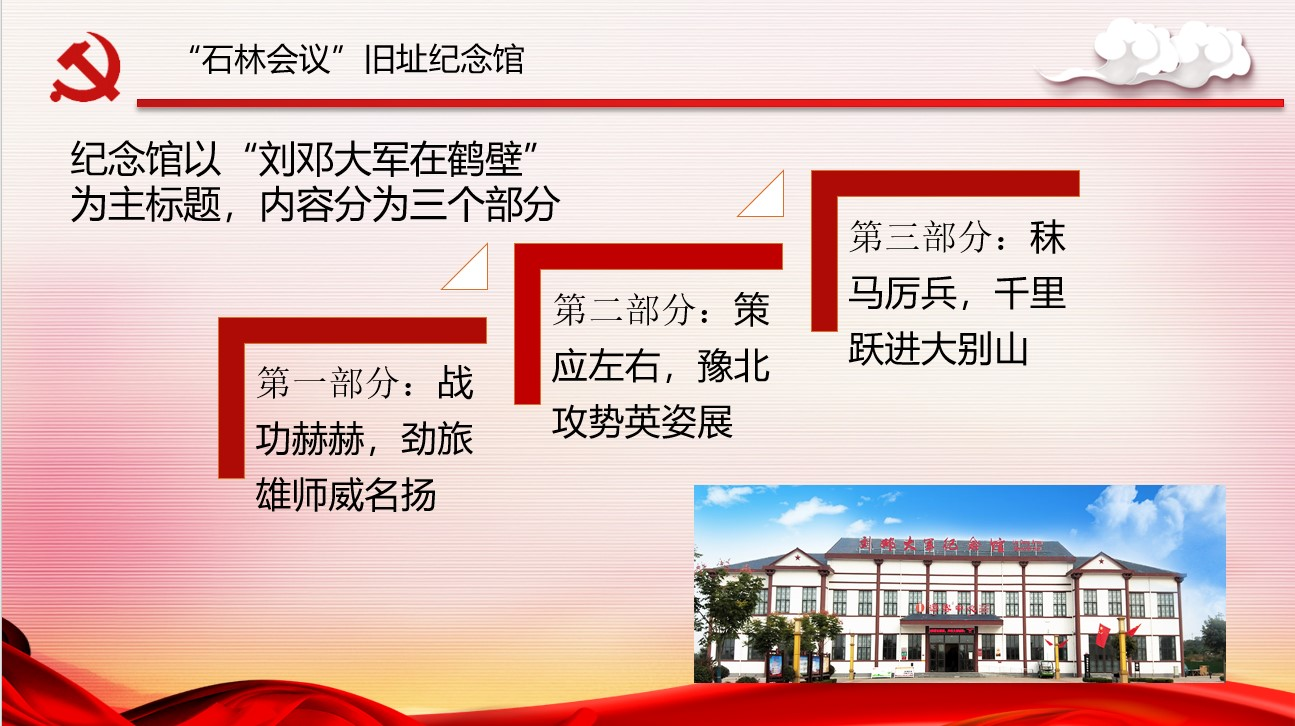
\includegraphics[width=7cm]{1.jpg}
    \label{(a)}
    }
    \quad
    \subfloat[]{
    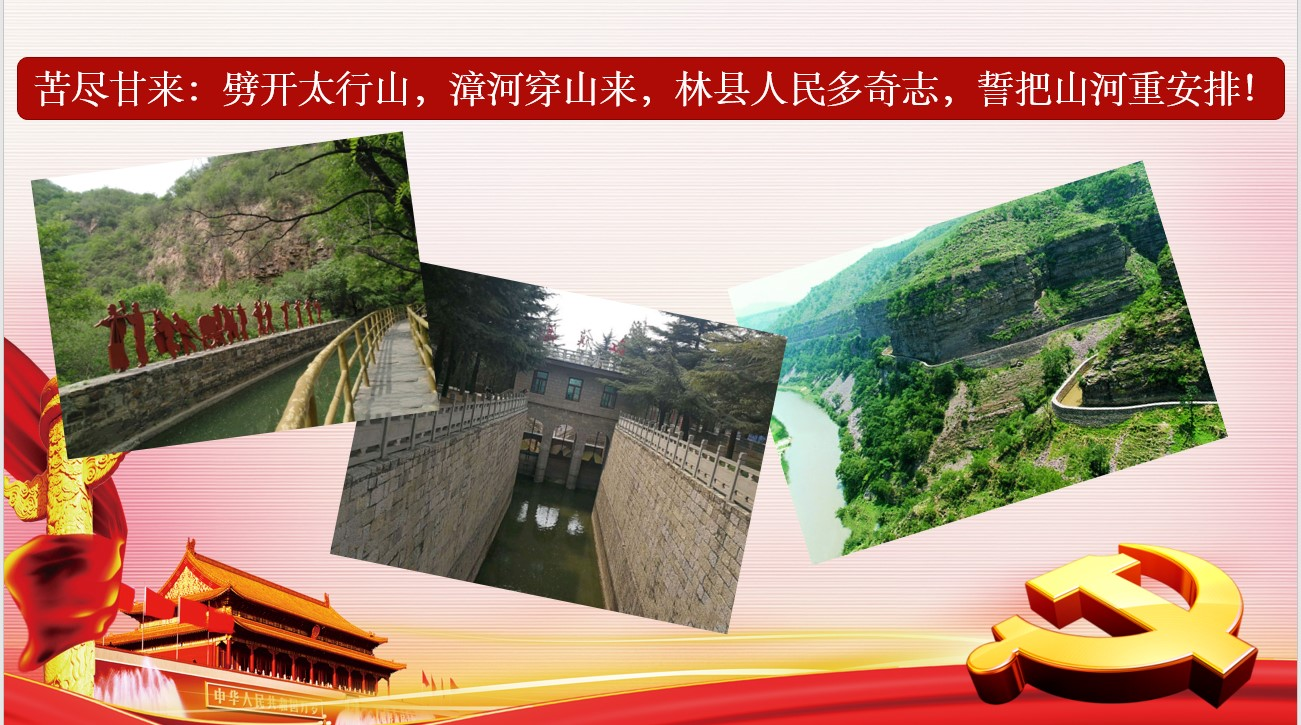
\includegraphics[width=7cm]{2.jpg}
    \label{(b)}
    }
    \quad
    \subfloat[]{
    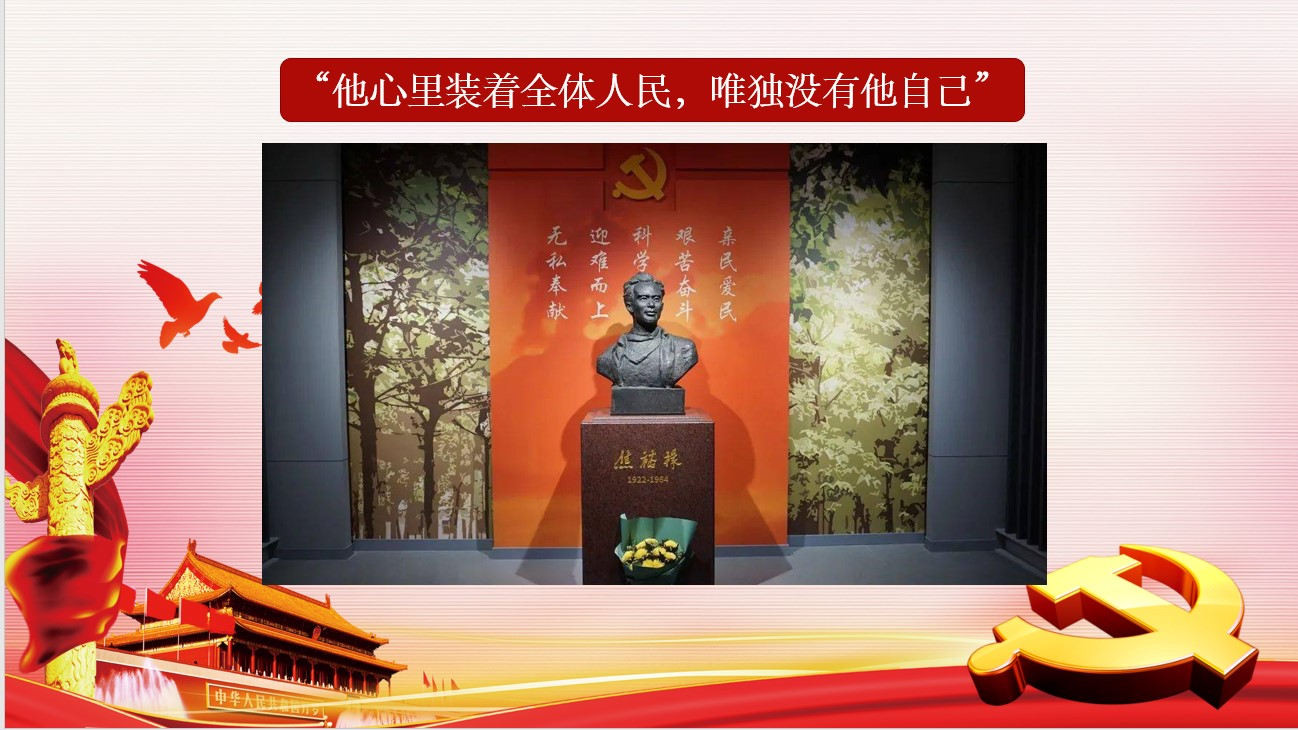
\includegraphics[width=7cm]{3.jpg}
    \label{(c)}
    }
    \quad
    \subfloat[]{
    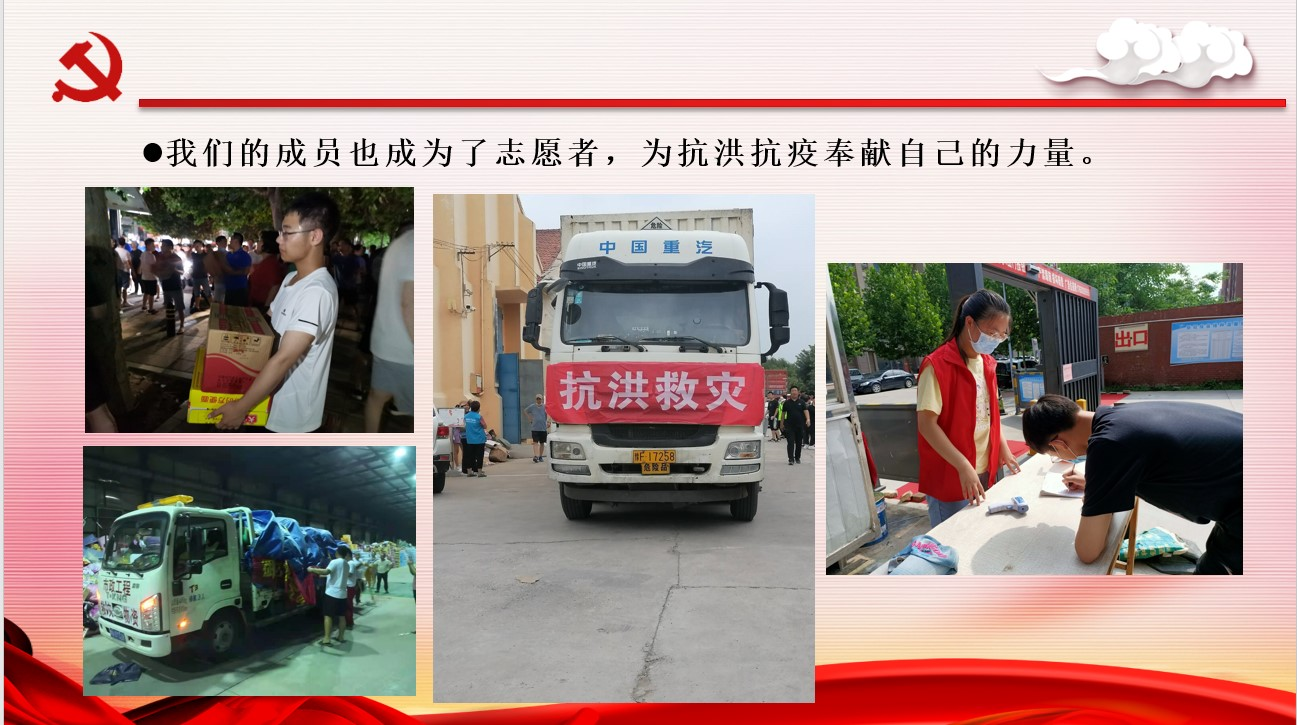
\includegraphics[width=7cm]{4.jpg}
    \label{(d)}
    }
    \caption{宣讲剪影}
\end{figure}
\begin{figure}[htbp]
    \centering
    \subfloat[]{
    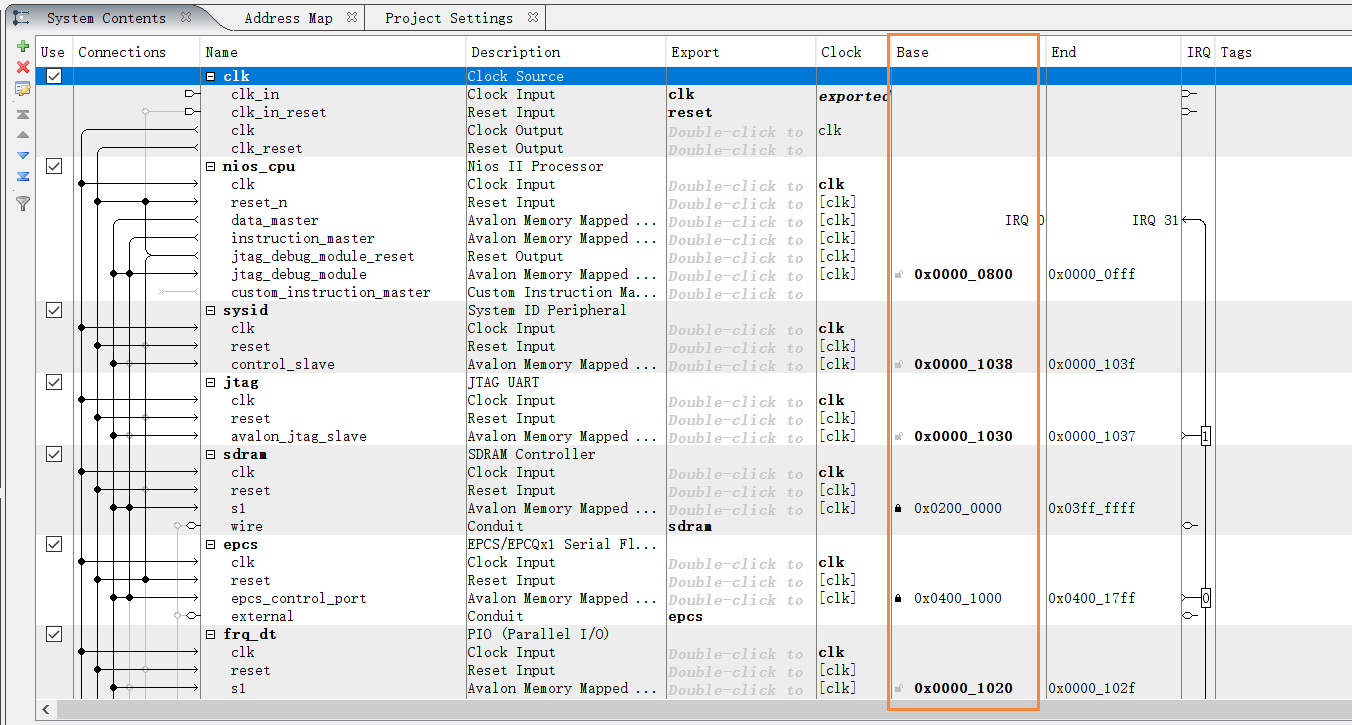
\includegraphics[width=7cm]{5.png}
    \label{(a)}
    }
    \quad
    \subfloat[]{
    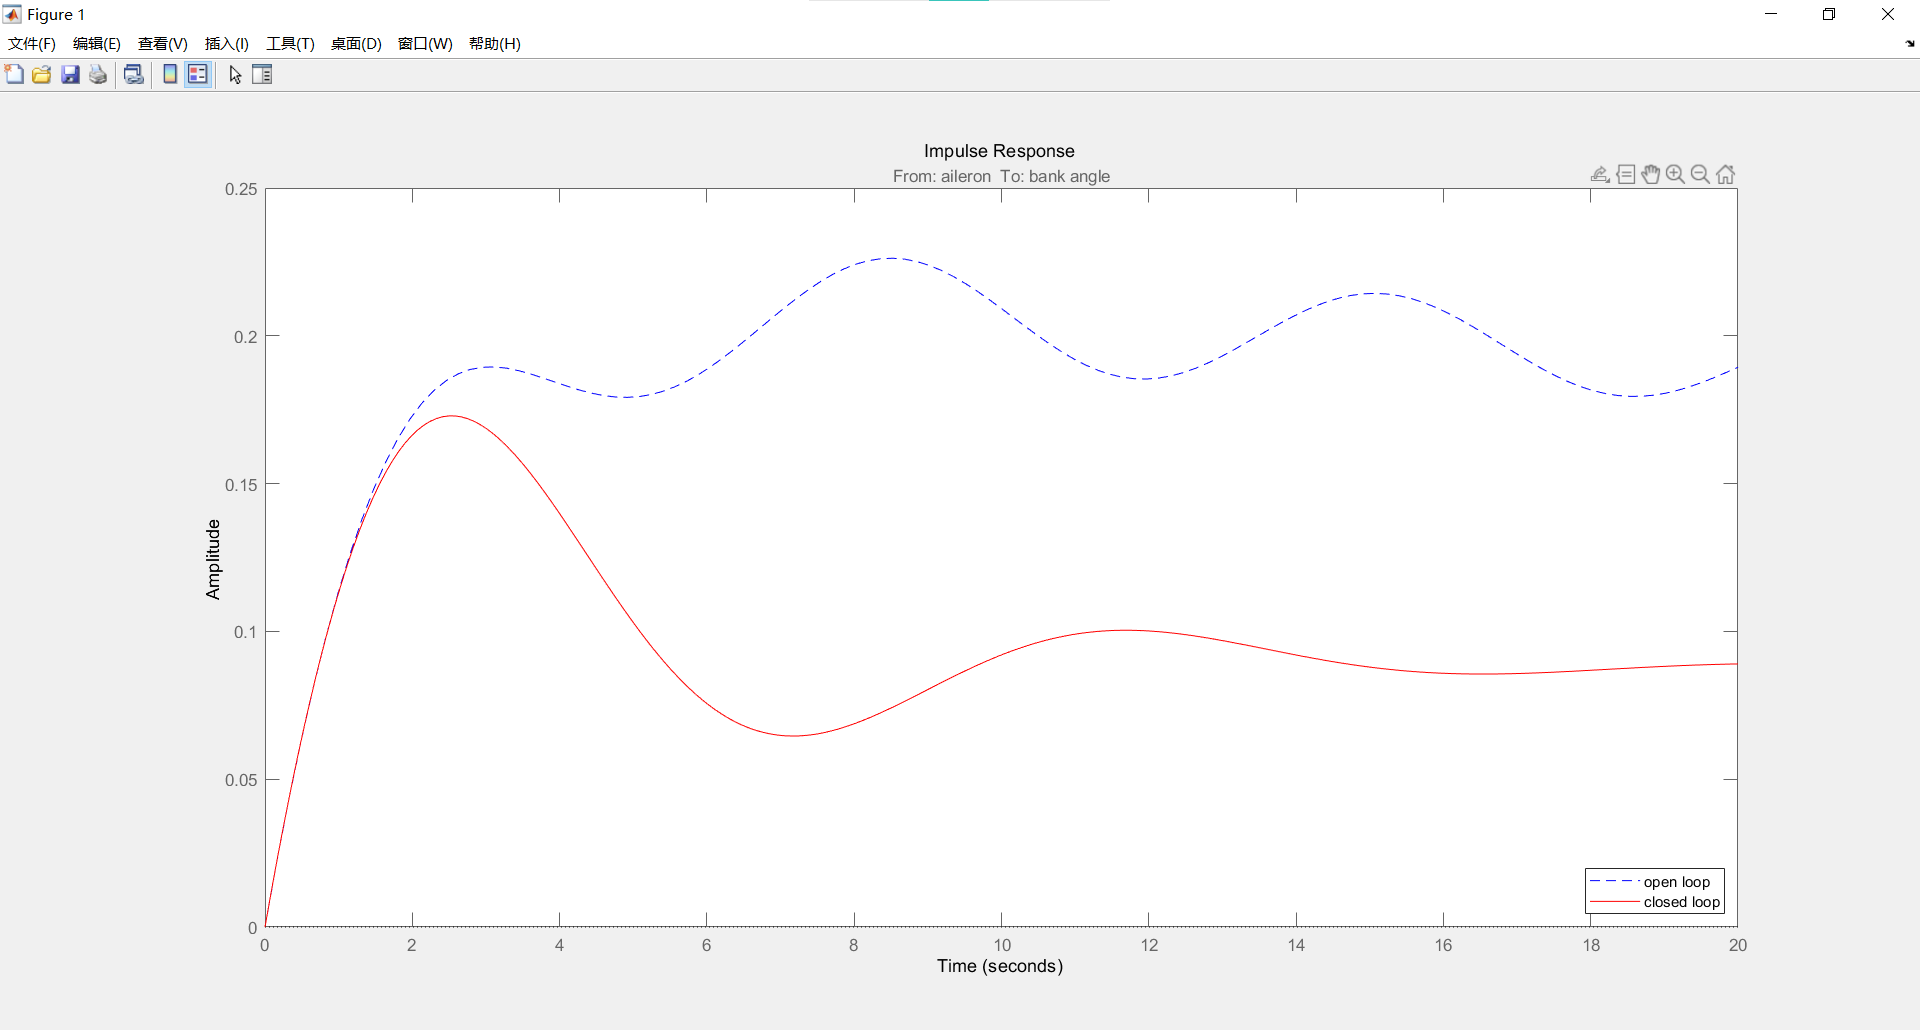
\includegraphics[width=7cm]{6.png}
    \label{(b)}
    }
    \caption{网站剪影}
\end{figure}
\begin{figure}[htbp]
    \centering
    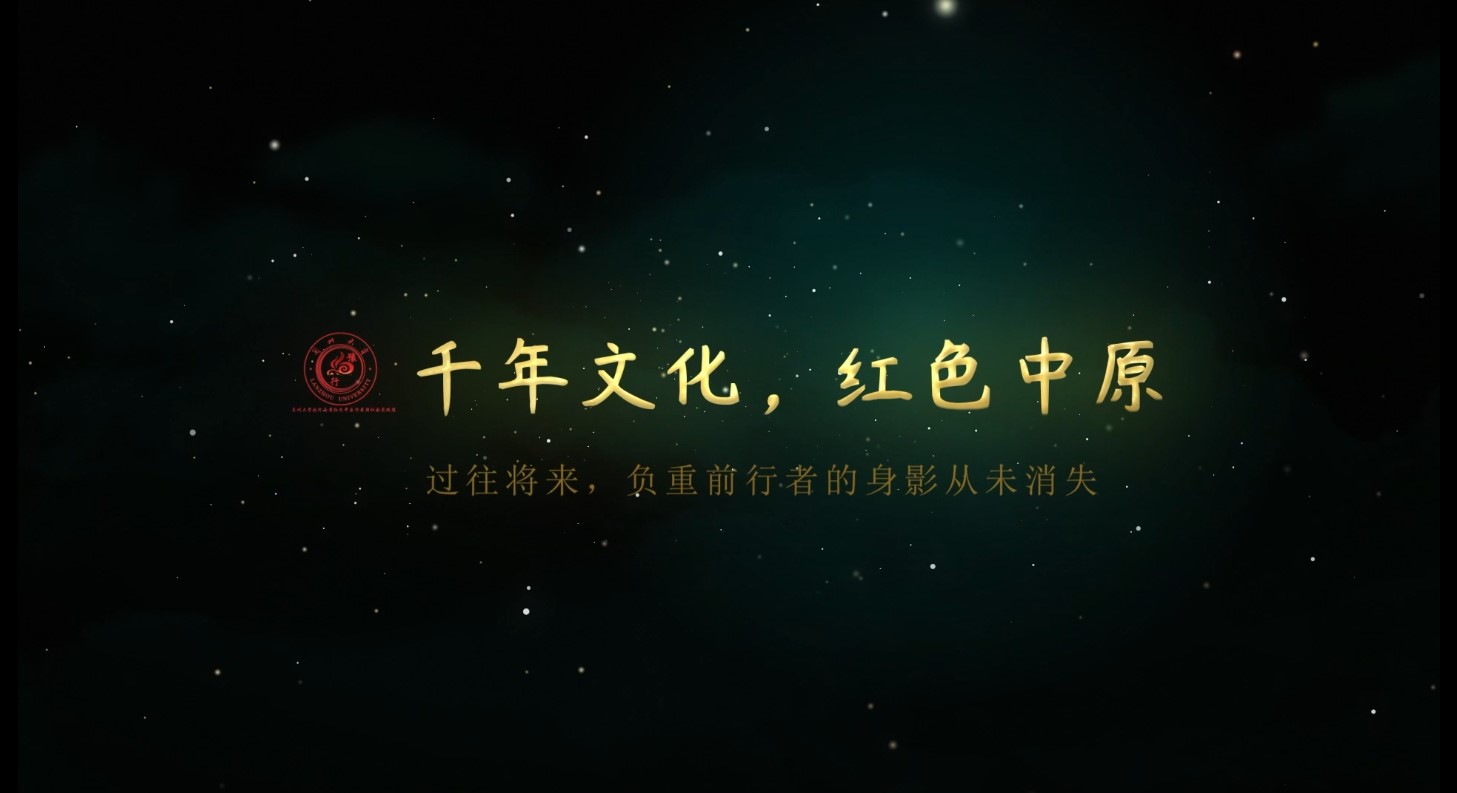
\includegraphics[width=500pt]{7.jpg}
    \caption{宣传视频剪影}
\end{figure}

\Thanks
团队指导老师马敏劲及全体暑期实践团队成员
\end{document}